\documentclass[11pt]{article}

\usepackage{subfigure,fancybox,epsfig,enumerate,amssymb,amsmath,amsthm,
fullpage,pst-plot,pstricks, arcs,tikz,hyperref,pstricks-add, graphicx}
\graphicspath{{images/}}


\newcommand{\A}{\ensuremath{\mathcal A}}
\newcommand{\B}{\ensuremath{\mathcal B}}
\newcommand{\F}{\ensuremath{\mathcal F}}
\newcommand{\C}{\ensuremath{\mathbb C}}
\newcommand{\K}{\ensuremath{\mathbb K}}
\newcommand{\R}{\ensuremath{\mathbb R}}
\newcommand{\Z}{\ensuremath{\mathbb Z}}
\newcommand{\defn}[1]{\textbf{#1}}
\newcommand{\ray}[1]{\overrightarrow{#1}}
\renewcommand{\line}[1]{\overleftrightarrow{#1}}
\newcommand{\segment}[1]{\overline{#1}}

\newtheorem{theorem}{Theorem}[section]
\newtheorem{lemma}[theorem]{Lemma}
\newtheorem{corollary}[theorem]{Corollary}
\newtheorem{claim}[theorem]{Claim}
\newtheorem{conjecture}[theorem]{Conjecture}
\newtheorem{prop}[theorem]{Proposition}


\theoremstyle{definition}
\newtheorem{definition}[]{Definition}
\newtheorem{observation}[theorem]{Observation}
\newtheorem{example}[theorem]{Example}
\newtheorem{note}[theorem]{Note}
\newtheorem{notation}[theorem]{Notation}
\newtheorem{ack}{Acknowledgements}
\newtheorem{axiom}{Axiom}
\newtheorem{problem}[theorem]{Problem}
\newtheorem{question}[theorem]{Question}
\newtheorem{aaxiom}{Axiom A}



\begin{document}
%This is where the fun begins!


\title{Josh \& Danny}

\maketitle

\section{Glide Reflections}
Now we will introduce the concept of a glide reflection, and prove which
combinations of isometries are equivalent to a single glide reflection.

%Possibly move this to section 1
\begin{definition}\label{orientation}
    The orientation of a plane is either positive or negative. We compute
    the orientation as follows: \\
    Pick 3 non-linear points in the plane $A$, $B$, and $C$. Let vectors
    $\ray{CA}$ and $\ray{CB}$ denote the vectors from $C$ to $A$ and $C$
    to $B$ respectively. The sign of the vector $\ray{CA} \times \ray{CB}$
    is the orientation.
\end{definition}

As we saw in a previous section, create any isometry of the plane where the
orientation is reversed can be made by three reflections. In the case where all
three lines are parallel, they can be reduced to a single reflection, and if
there is only one intersection point, they are one reflection line, but in the
case where there are at least two points of intersection among the lines of
reflection, they represent an operation that cannot be reduced into a single
one of any of the isometries that we have introduced; therefore we will reduce
them to a representation where each isometry has a unique identity and refer to
this class of isometries as glide reflections.

\begin{definition}\label{glide reflection}
  A glide reflection is a form of isometry represented by a composition of a
reflection and a translation parallel to the line of reflection; it is a
fundamental isometry which is distinct from the other three.
\end{definition}

The fundamental nature of a glide reflection will be easy to see, but first we
will look at how a glide reflection can be formed from three reflections, as
this will demonstrate the reasons for our choice of representation.

\begin{theorem}\label{3 reflections form a glide reflection}
  A glide reflection is formed by the composition of three reflections that
  have at least two points of intersection among them.
\end{theorem}

First we will consider the case where two of the reflection lines are parallel,
but first we need a supporting theorem which will be required to completely
reduce the reflections:

\begin{theorem}\label{glide reflection from a reflection and a translation}
  A glide reflection can be formed from one reflection and one translation,
  as long as the angle between the reflection line and translation vector is
  not 90 degrees.
\end{theorem}

\begin{proof}
  A reflection and a translation perpendicular to each other can be combined by
  moving the reflection by half of the translation's magnitude in the opposite
  direction.

  Therefore, a reflection line and a translation vector with an arbitrary angle
  between them can be reduced to a glide reflection by taking the components of
  the translation vector both parallel and perpendicular to the reflection
  line, which compose to form the first translation; the perpendicular
  component can be absorbed by moving the reflection line, and since the
  parallel component must be non-zero due to the restriction on the angle of
  the translation vector, the remaining two isometries make up our definition
  of a glide reflection.
\end{proof}

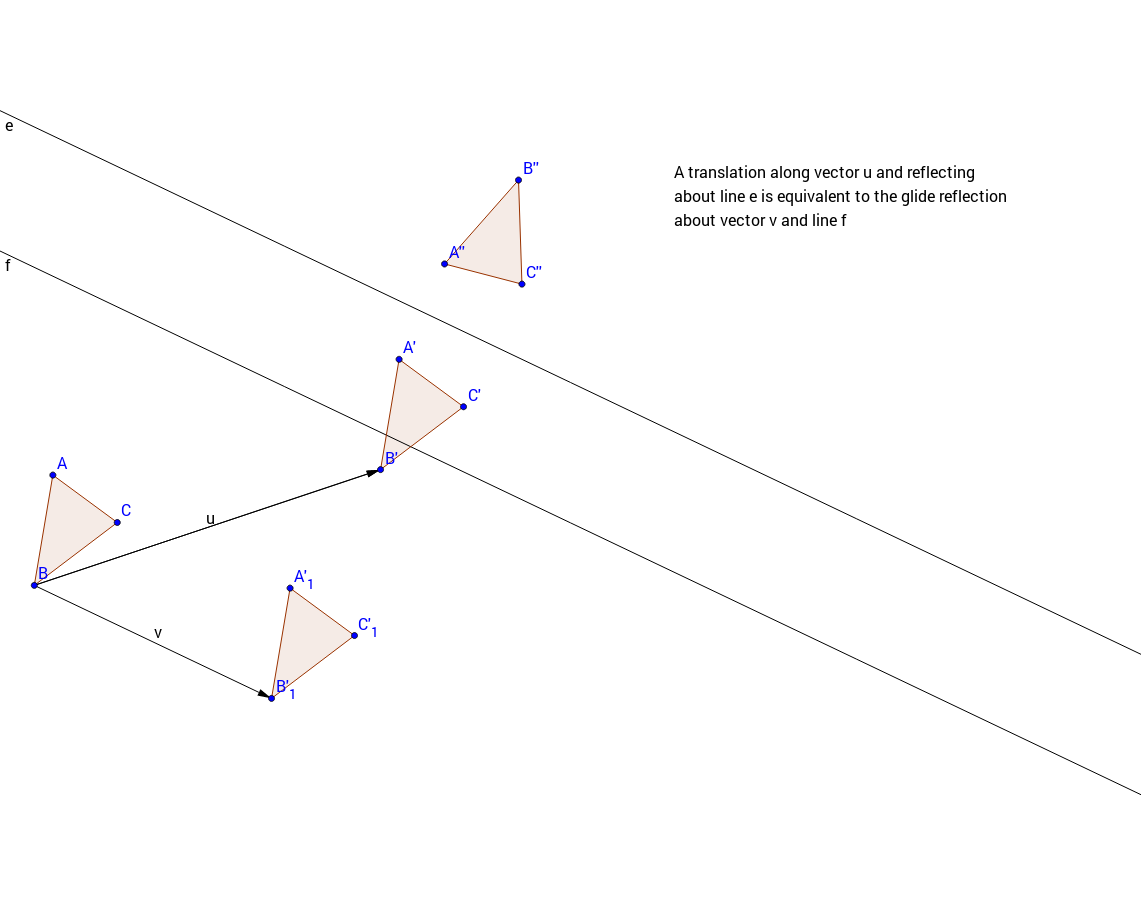
\includegraphics[scale=.4]{glide}

Now we can prove Theorem 5.1 for the following case:

\begin{proof}
  For a set of reflection lines $L_{1}$, $L_{2}$, and $L_{3}$, where the first
  two are parallel and the third intersects both, the composition is a glide
  reflection since the parallel reflection lines, $L_{1}$ and $L_{2}$, are a
  single translation. The resulting translation vector will never be at a 90
  degree angle with the remaining reflection line, $L_{3}$, because that
  reflection line started off at some angle with respect to $L_{1}$ and
  $L_{2}$, and as shown above, this forms a glide reflection.
\end{proof}

In order to show that any three reflections can be made into a glide
reflection even if none are parallel, we leverage the fact that two
intersecting reflections form a rotation.

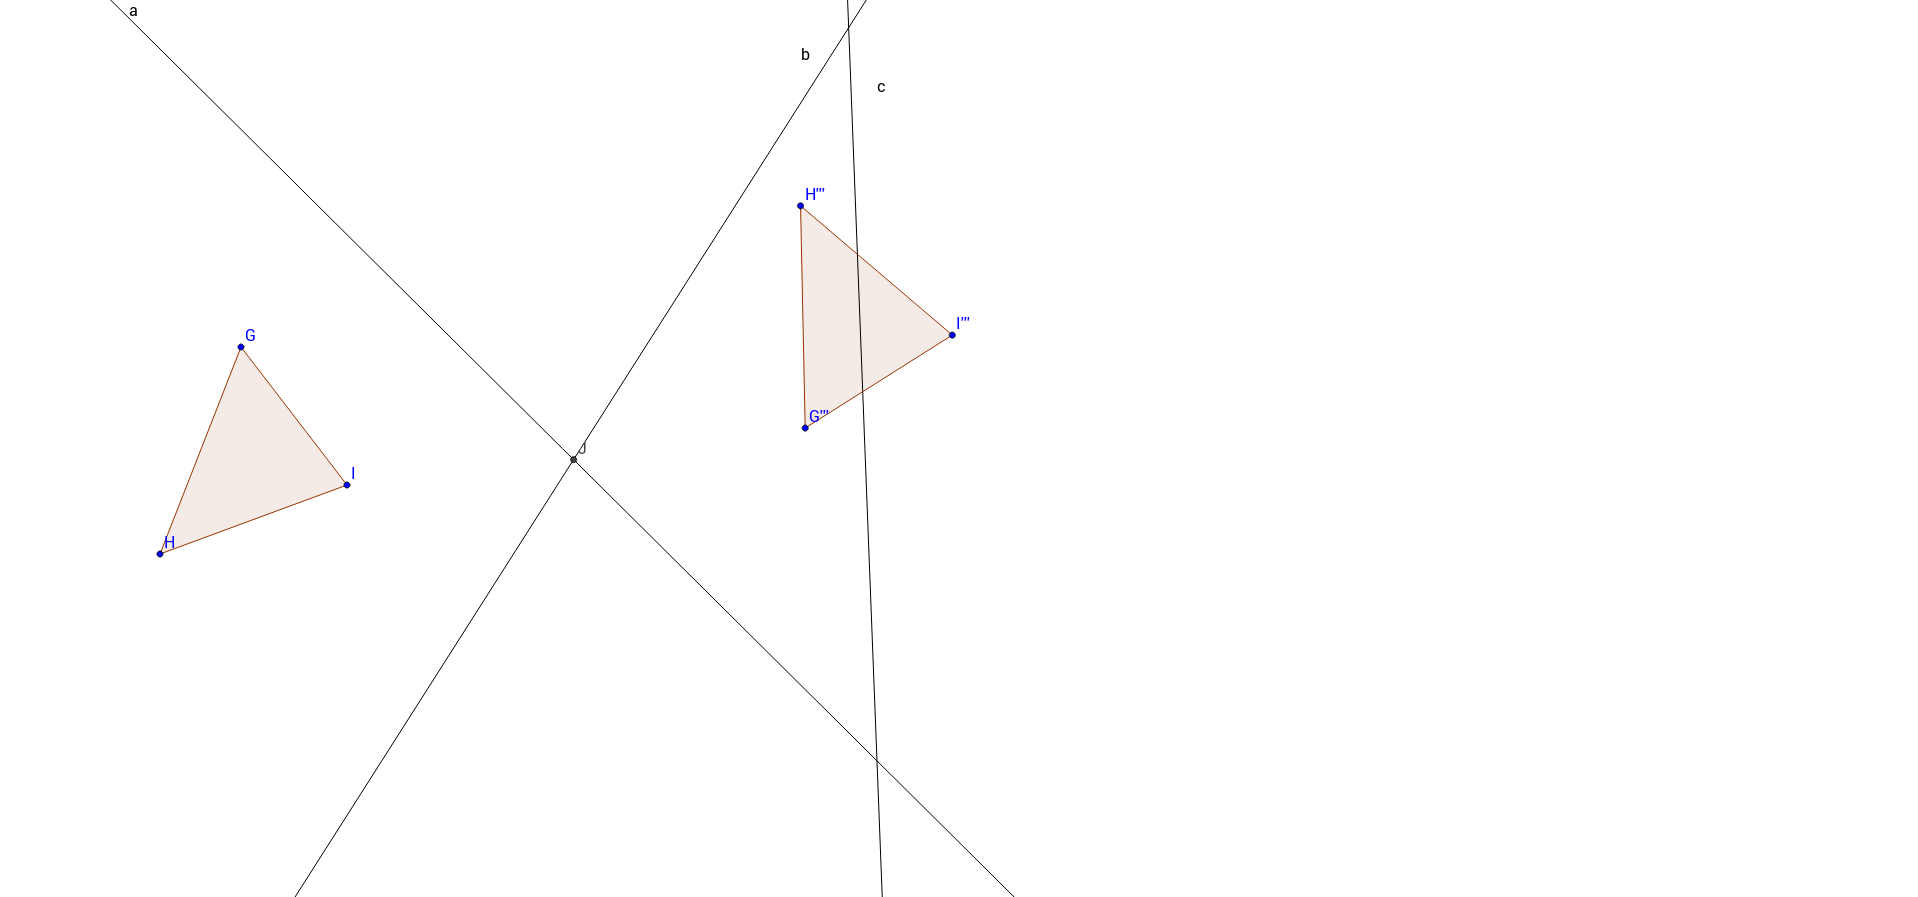
\includegraphics[scale=.4]{intersect3}
\begin{proof}
  For a set of reflections across lines $L_{1}$, $L_{2}$, and $L_{3}$, where
  there are exactly three intersection points, the isometries can be reduced to
  a glide reflection by rotating two of the reflection lines such that one of
  them is parallel to the third. This can be done because two intersecting
  reflection lines compose to form a rotation around the intersection point:
  first transform the two reflections into the rotation, then choose a new
  reflection line through the center of rotation that is parallel to the third
  reflection line. It is guaranteed that a reflection line exists such that
  when composed with the reflection line that you chose it will reproduce the
  rotation around that center point. Now that the lines that formed the
  rotation have been transformed, you have reached the case where two
  reflection lines are parallel and the third intersects both, which we have
  already shown to be a glide reflection.

\end{proof}
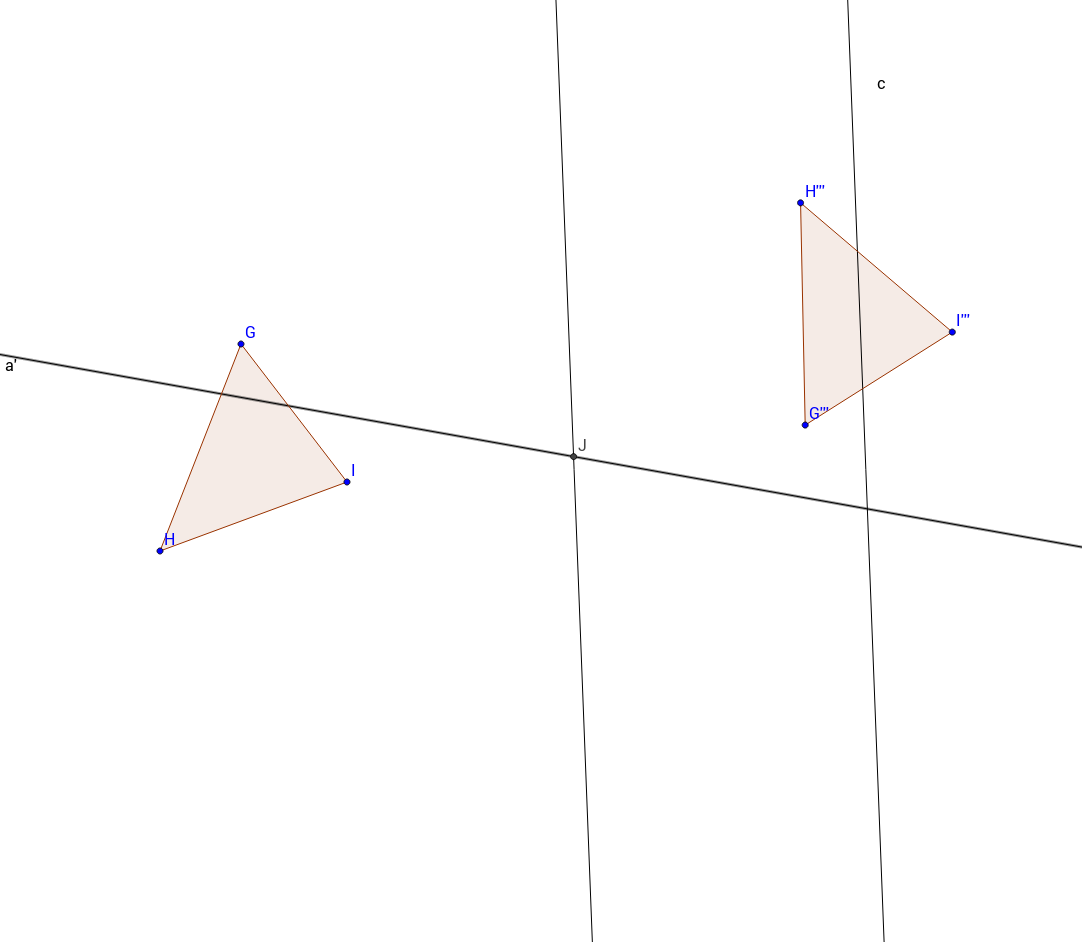
\includegraphics[scale=.4]{intersect21}

\subsection{Exercises}

Now that we've introduced the concept of glide reflections, there are a few
things which can increase your understanding of them and other isometries:
\begin{enumerate}
\item Add a column for "glide reflections" to your composition table. Are there
  compositions you couldn't do before that are simpler with glide reflections?
  What sorts of compositions can you have with glide reflections?
\item prove that the reflection and translation used to make a glide reflection
  commute with each other, so there is no need for ordering them.
\item Why do we require the translation to be parallel to the reflection line?
  What properties do we gain by doing so? What would it mean for glide
  reflections if we didn't require this?
\item Think about how to find the isometries you get when there are less than
  two points of intersection.
\end{enumerate}

\end{document}
